\documentclass[../physical_computing.tex]{subfiles}

\begin{document}

\chapter{Calculations with Negative Integers and Real Numbers}
\label{ch:arithmetic}

\subsection{Negative Integers}
\label{sec:negatives}

What about if we have negative integers? These are almost always represented using a method called twos complement. Suppose we have 4 bits in our binary representation. So far we have thought of these as representing the unsigned integers between 0 and 15. However, recall that the binary number $B1111$, neglecting overflows, is adjacent to the binary number $B0000$. How about using $B1111$ to represent -1? Following the same logic, $B1110$ is adjacent to $B1111$, so it must be -2. Carrying on with this argument, we reach a binary four-bit twos complement representation for the signed integers in the range $[-Do you understand the meaning of Wouter's question here? I'm thinking he has submitted his receipts and is wondering if he has to do anything else to get reimbursed, and probably how long it is likely to take? I'm asking because we are of course trying to hire this guy, soDo you understand the meaning of Wouter's question here? I'm thinking he has submitted his receipts and is wondering if he has to do anything else to get reimbursed, and probably how long it is likely to take? I'm asking because we are of course trying to hire this guy, so8,+7]$,

\begin{table}[hbt]
    \centering
    \begin{tabular}{|c|c|c|}
    \hline
         decimal & binary & hexadecimal \\
         \hline\hline
         0 & B0000 & 0x0 \\
         1 & B0001 & 0x1 \\
         2 & B0010 & 0x2 \\
         3 & B0011 & 0x3 \\
         4 & B0100 & 0x4 Do you understand the meaning of Wouter's question here? I'm thinking he has submitted his receipts and is wondering if he has to do anything else to get reimbursed, and probably how long it is likely to take? I'm asking because we are of course trying to hire this guy, so\\
         5 & B0101 & 0x5 \\
         6 & B0110 & 0x6 \\
         7 & B0111 & 0x7 \\
         -8 & B1000 & 0x8 \\
         -7 & B1001 & 0x9 \\
         -6 & B1010 & 0xa \\
         -5 & B1011 & 0xb \\
         -4 & B1100 & 0xc \\
         -3 & B1101 & 0xd \\
         -2 & B1110 & 0xe \\
         -1 & B1111 & 0xf \\
        \hline
    \end{tabular}
    \caption{Decimal, binary and hexadecimal symbols for the twos complement representation of the signed integers in the range $-8$ to $+7$ inclusive.}
    \label{tab:twoscomplement}
\end{table}

You might notice that moving from $-1$ to $-8$ is a binary count upwards but with the symbols $1$ and $0$ reversed. This means that there is a simple logical way to deduce the binary representation of $-x$ from the binary representation of $+x$. This is
\begin{align}
    -x=\neg x+1.
\end{align}
Let us check that this works. For example, the binary representation of 3 is $B0011$. We take the bitwise not of this binary sequence to get $B1100$, then we add one to this to get $B1101$. From Table \ref{tab:twoscomplement} this represent -3. Try a couple of others. Note that it won't work for -8, because +8 cannot be represented in twos complement signed integer arithmetic using only four bits.

\subsection{Integer addition and multiplication}
\label{sec:addmultiply}

I am about to teach you how to add and multiply binary numbers by hand as you might have learned to do in school for decimal numbers. Of course, there are calculators that have a binary mode - indeed, yours probably does. You can do your binary calculations there, or check your manual calculations using them. There are also online binary and hexadecimal calculators - see, for example \url{calculator.net/binary-calculator.html}.

When you were at school you were probably taught about column addition as a way of adding together two numbers each of which had multiple non-zero digits. You basically write out the two numbers one above the other with each succesive digit aligning vertically with the other number to be added. You then add the digits in the corresponding columns starting with the least significant digit and moving across until you have done the most significant one. The interesting case is when the sum of the two digits exceeds the capacity of the symbols available from a single digit. In this case you 'carry' the difference to the next column, usually writing the carried number below the output to remind you to add it on when you get to the next column. If there are any carry digits left at the end, these are added on the left. 

It's almost the same thinking about binary addition, except the 'columns' instead of being $1$, $10$, $100$ etc are $1$, $2$, $4$, $\cdots$. In both cases, the M\textsuperscript{th} column represents $\rm (base)^{(M-1)}$. The only other modification is that you methodically {\it ignore the overflows}. Let us do some examples. For a start, $2+3$ or $B0010+B0011$. Figure \ref{fig:addition_example_1} shows how this is carried out using column addition.
\begin{figure}[h!]
    \centering
    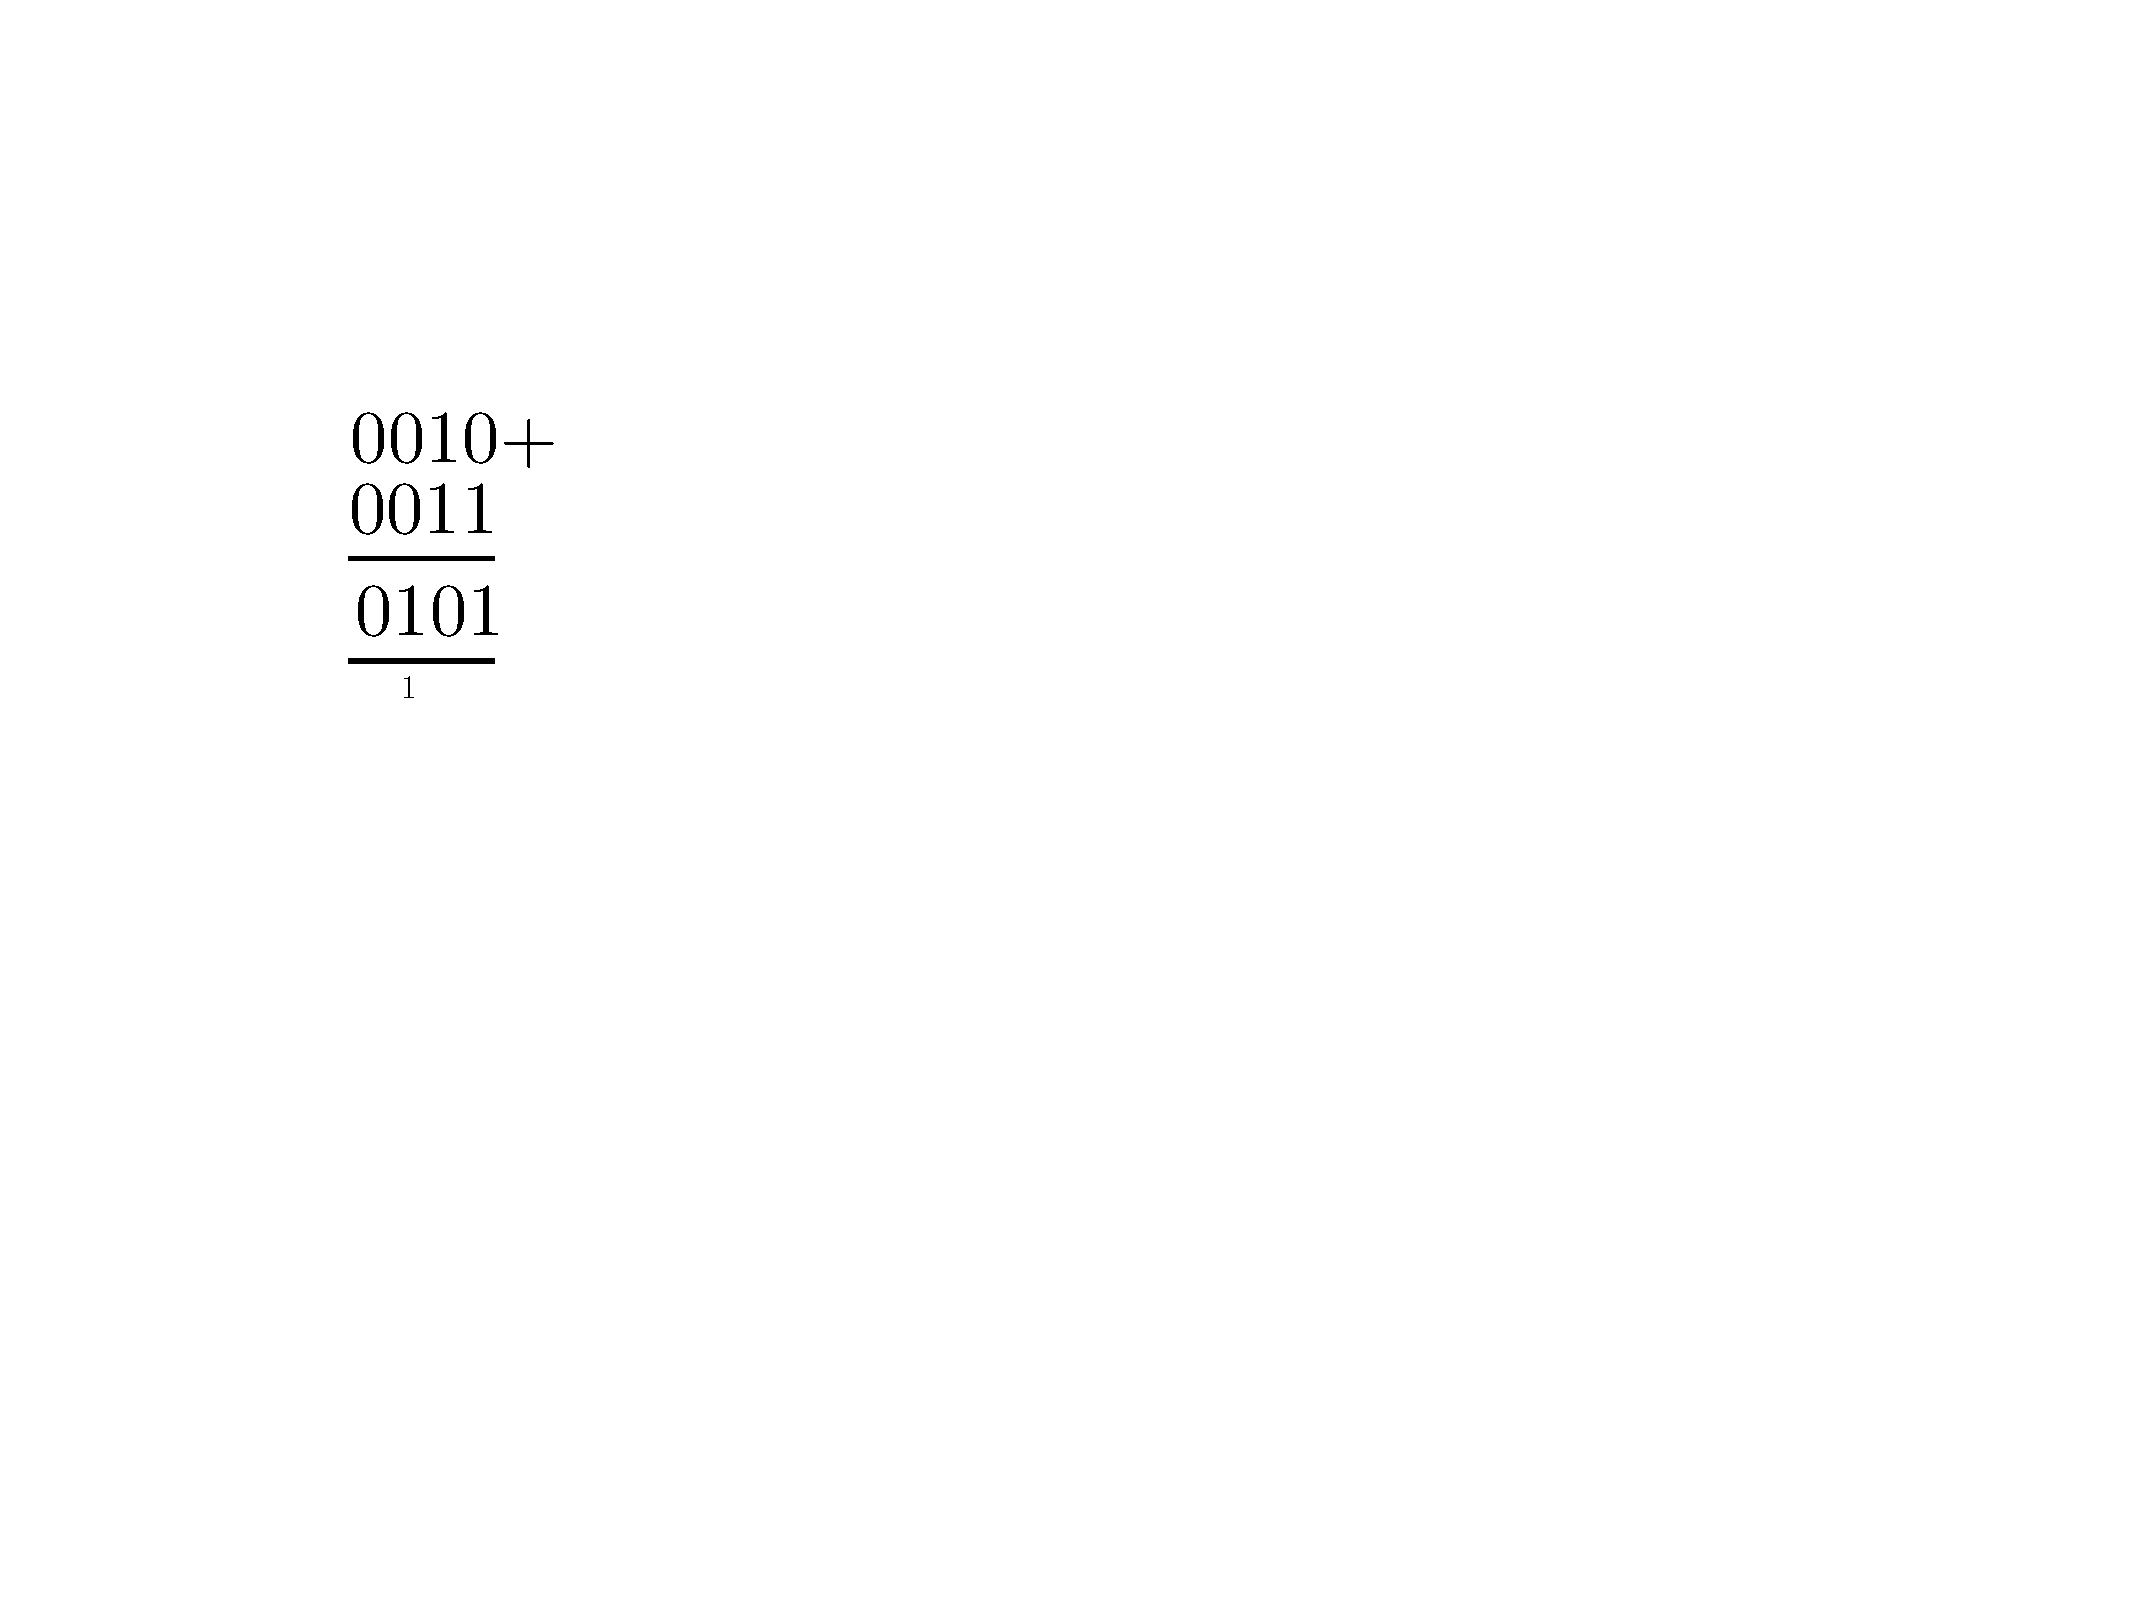
\includegraphics[width=0.1\textwidth]{figures/addition_example_1.pdf}
    \caption{Adding 2 and 3 in binary.}
    \label{fig:addition_example_1}
\end{figure}
In this example, the second column addition results in a carry of $B1$ to the third column, and the third column then just contains that $B1$, so that the overall answer is $1$ times $2^2$ + $1$ times $2^0$, or five.

In the next example, shown in Figure \ref{fig:addition_example_2}, we carry out $-3+7$. The four bit binary representation of $+7$ is $B0111$. To obtain the binary representation of $-3$ we start with $+3$ which is $B0011$. We first do a bitwise not, leading to $B1100$, then we add a least significant bit, $B0001$, to obtain $B1101$, and that's our four-bit binary representation of $-3$. Finally, we carry out the column addition. Notice that when we get the answer we truncate at 4 bits, discarding the overflow $1$. This leads to the correct binary representation of the answer, $B0100$, which is +4.
\begin{figure}[h!]
    \centering
    
\includegraphics[width=0.1\textwidth]{figures/addition_example_2.pdf}
    \caption{Addition of $-3$ and $+7$ in binary}
    \label{fig:addition_example_2}
\end{figure}
For a final example of addition, let us consider $2-4$. We do this subtraction by considering it as $2+(-4)$, and then working out the twos complement representation of $-4$. To do this, start with $+4$, which is $B0100$, perform a bitwise not to obtain $B1011$, and add one LSB to obtain $B1100$. The addition is then carried out as shown in Figure \ref{fig:addition_example_3}. There turn out to be no carry bits necessary in this sum, and the resulting binary $B1110$ is $-2$ in decimal, as can be found out by subtracting $1$LSB to obtain $B1101$ and doing the bitwise not to obtain $B0010$, which is $+2$, hence the original $B1110$ must be $-2$. This is also confirmed by Table \ref{tab:twoscomplement}.
\begin{figure}[h!]
    \centering
    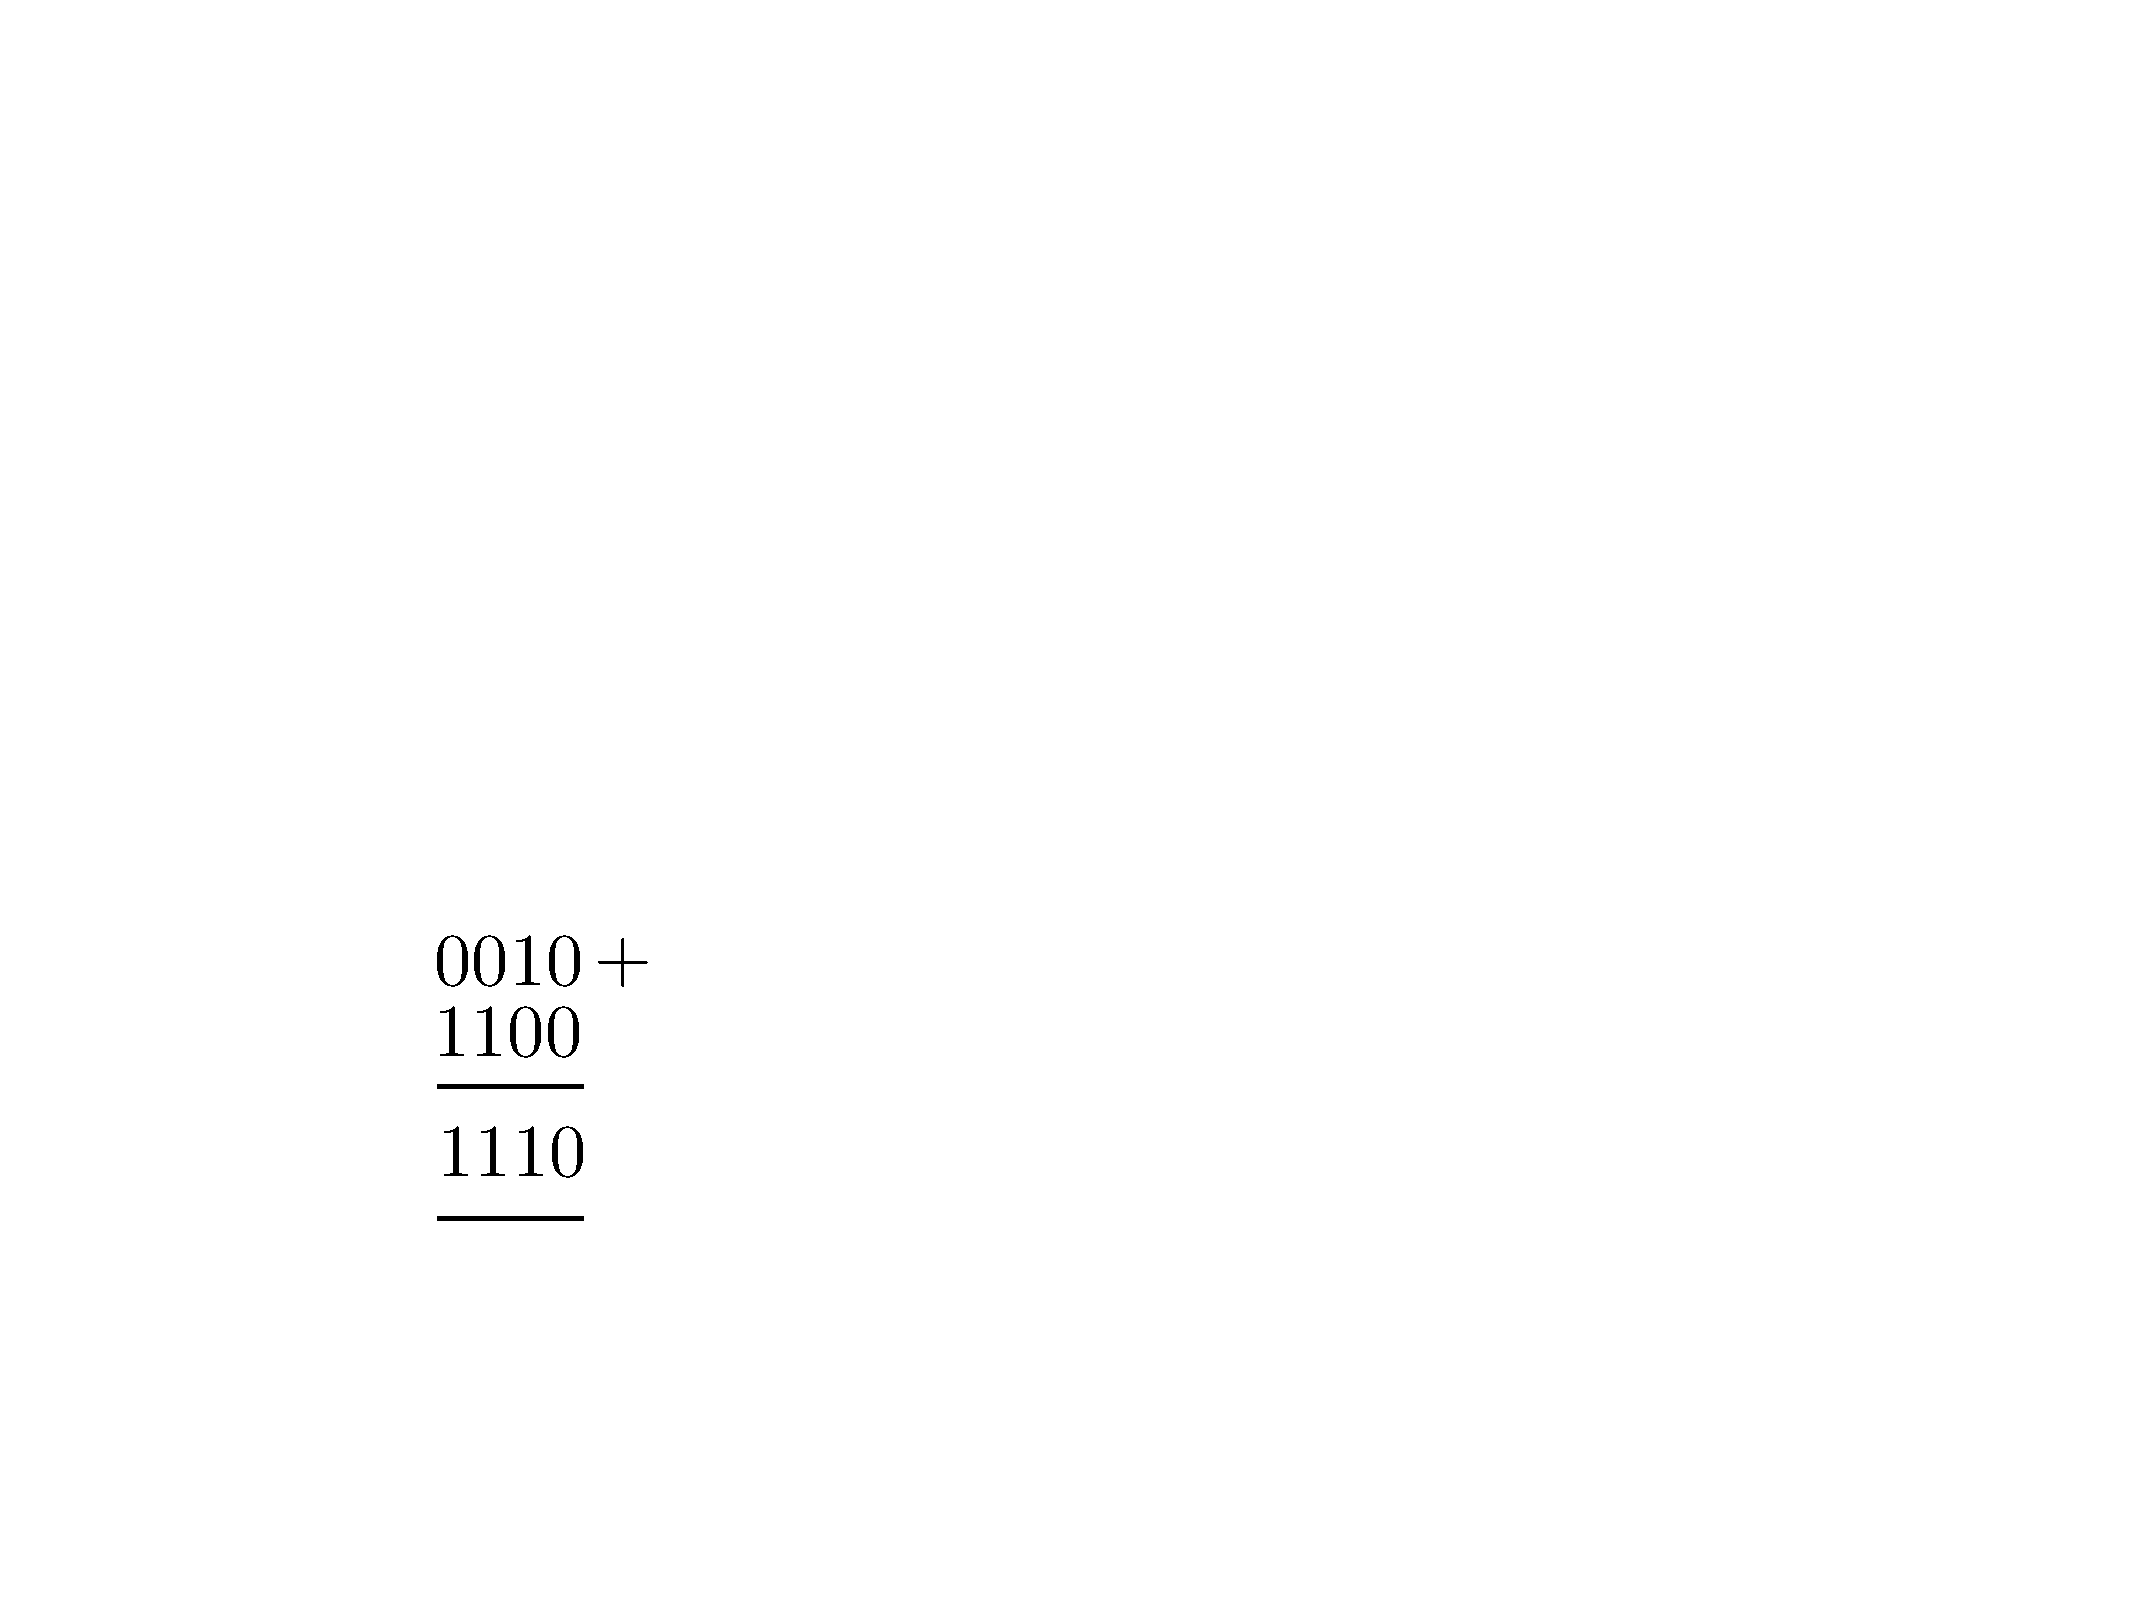
\includegraphics[width=0.1\textwidth]{figures/addition_example_3.pdf}
    \caption{The addition of $+2$ and $-4$.}
    \label{fig:addition_example_3}
\end{figure}

Next we move on to multiplication, which is carried out using the columnwise long multiplication technique you were taught in school. An example is shown in Figure \ref{fig:multiplication_example_1}.
\begin{figure}[h!]
    \centering
    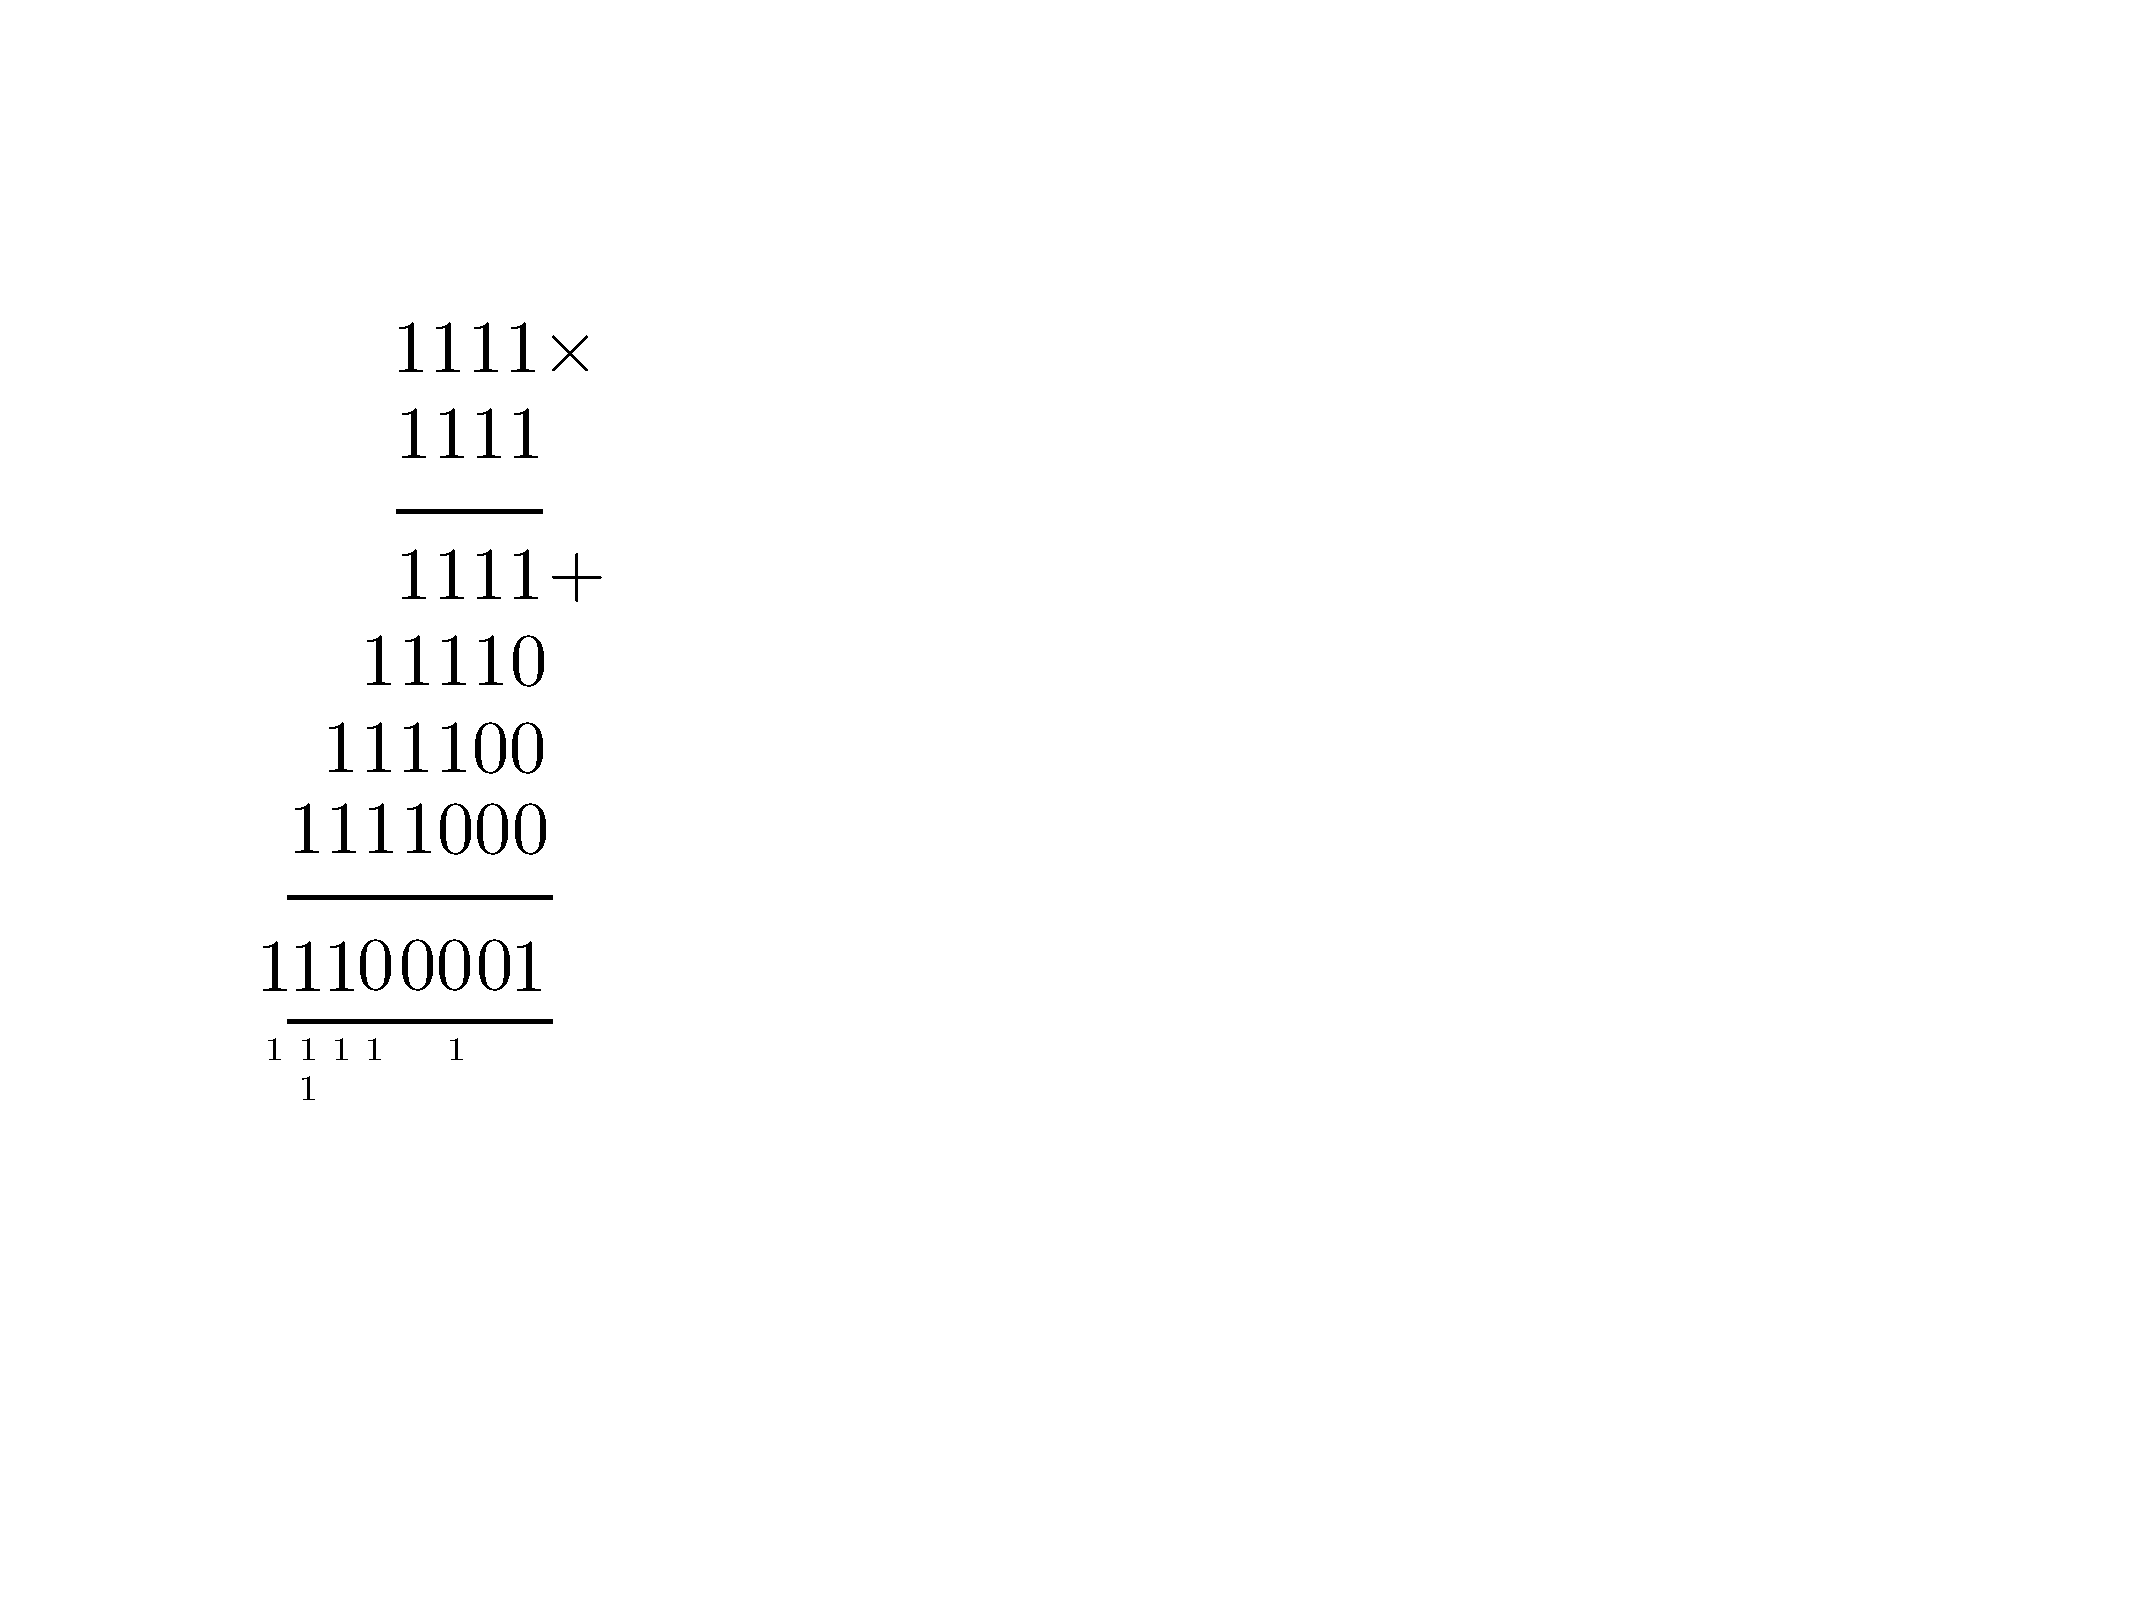
\includegraphics[width=0.18\textwidth]{figures/multiplication_example_1.pdf}
    \caption{Multiplication of the four bit representation of $-1$ by itself.}
    \label{fig:multiplication_example_1}
\end{figure}
The two inputs are $B1111$, which is the 4-bit twos complement representation of $-1$. We expect to obtain $-1\times-1=+1$. We proceed as we do in decimal long multiplication. First the least significant bit of the second number by all digits of the first one, placing the result on the top output row. Some notation if you haven't encountered it: a `leading' digit is one to the left of all the digits visible in a set of digits; a `trailing' digit is one to the right of those digits. Now add a trailing zero to the LSB of the next row, then proceed to multiply the second least significant bit of the second input number by the first row, and place the binary result to the left of the trailing zero. Repeat with the other two bits of the second input number. You will now have four rows containing binary numbers with one more bit in each successive row. Add the four rows up. 

When adding the four rows up we will encounter an oddity of addition that isn't often encountered in decimal column addition, although it can also happen. In the later columns, there end up being in some cases four or more $1$s to add. In these cases the result has more than two digits in binary. For example, in binary $B1+B1+B1+B1=B100$. In these cases you end up adding carry digits to other columns than that immediately to the left of the one you are working on. In the case of a $B100$ result in a column addition, you'd need to add a carry $1$ to the column two to the left of the current. And so on. In some cases there will end up being multiple carry $1$s in a column. This happens in in column 7 of the example. 

In fact, you only need to carry out sufficient columns of the multiplication and subsequent addition to get the result for the four least significant bits of the long multiply, because all higher bits are going to be discarded. The result, truncating to four bits, is $B0001$, so that in 4-bit twos complement binary $-1\times-1=+1$. So, everything seems consistent.

\section{Sign-extension}
\label{sec:signextension}

It often happens that you want to multiply two numbers represented
in some N-bit binary representation, and it is clear that the 
result is going to require more than N bits to represent it. 
When this happens, it is necessary to add more bits to the left
of the MSB in each of the input numbers. If you are using 
an unsigned representation, you just add zeros. However, if you
are in a twos complement signed representation, and the input 
number is negative, then the leftmost bit will be $1$. It turns
out that if you pad negative numbers, those with a leftmost $1$, 
with $1$'s to the left, then this maintains the binary number
as having the same numerical value in the expanded representation
with more bits, just as padding a positive binary number with 
zeros to the left maintains its value. This procedure of padding
based on the value of the most significant bit is called 
sign extension. The same rule applies to real numbers with 
fractional parts, which we discuss next.

\section{Fixed point arithmetic with real numbers}
\label{sec:fixedpoint}

Real numbers that are not integers, can be multiplied and added together using the same rules as described above, with three
additional new elements. The representation we arrive at 
after adding these elements is known as fixed point representation.
It is somewhat of a misnomer, because there is no
point in a binary sequence, and because the position of 
$2^0$ does in fact move around between columns as we shall
see. The terminology makes sense in the context of the 
popular floating point representation of numbers, where the 
position of the $2^0$ column is recorded in a second binary 
number, the exponent. Floating point numbers are in practice
tricky to manipulate digitally due to the large number of
special cases that are necessary to represent all the 
possible numbers in a range, so a discussion of them is beyond
the scope of this book. You can read about floating point
representation of numbers in \cite{Warren:10.5555/2462741}, 
chapter 17.

The first rule concerns how to represent the fractional 
portion of numbers. 
We are free to interpret any one of a sequence of bits
as representing the number $1=2^0$. When representing
integers, the rightmost bit
has been $1$, but if we were to make, say the third-rightmost
bit equal to $1=2^0$, then the bit to the right of it would 
be $2^{-1}=0.5$ and the LSB would be $2^{-2}$. In this 
representation, the smallest positive number that could be 
represented by the string of binary numbers would be $0.25$,
Let's say we have six bits in our number system, and let us 
say we wish to represent positive as well as negative real 
numbers. The largest positive number is represented by 
$011111$, which is $4+2+1+0.5+0.25=+7.75$. To find 
the representation of $-7.75$, do $\neg{B011111}+1{\rm LSB}$, 
which is $B100000+1{\rm LSB}=B100001$. The binary string for
$-0.25$ in this representation is $B111111$, since the smallest
negative number is all 1s. If we add this to the representation
of $-7.75=B100001$ and discard the overflow, we obtain
$B100000$, so the most negative number representable in six
bit twos-complement binary with $2^0$ represented by a 1
in the third-from-rightmost bit column is $-8$.

The second rule concerns how to work out the representation of
the answer. In addition, you ensure that the columns where
$1=2^0$ is written are the same in both inputs, and you follow
the same rule as for addition of signed integers, discarding any 
overflows in the result. For multiplication, you line up the
$2^0$ columns as before. In the result, the rule is that you
add the number of columns to the right of $2^0$ in the two 
inputs, and the sum of these numbers of columns is the number of
columns to the right of $2^0=1$ in the result. This exact same
rule is used to position the decimal point in 
the answer to the product of two decimal numbers.

\section{A fixed point multiplication example}
\label{sec:minusfourandaquarter}

Let us say we wanted to compute $-4.25^2$ in binary. In the
same 6-bit fixed point representation discussed in 
Section \ref{sec:fixedpoint}, $+4.25$ is $B010001$. We
find $-4.25$ by doing $\neg(B010001)+1{\rm LSB}$, which
is $B101110+1{\rm LSB}=B101111$. Next, we recognise that
we will probably need some more bits, so let's just
add another six bits to the right by sign extension,
so that we end up with a 12 bit representation of
$-4.25$, which is $B111111101111={\rm 0xfef}$. Not
wanting to do a tortuous long multiplication, I use
a web-based binary calculator to do the heavy lifting,
taking only the 12 least significant bits of the result, and I 
obtain $B000100100001={\rm 0x121}$.
Following the rule that you add the 
number of digits to the right of $1$ in each of the inputs,
there are $2+2=4$ digits to the right of 1 in this number,
so that the LSB represents $2^{-4}=0.0625$, which is 1/16.
The digits other two non-zero digits are 2 and 16, so the 
answer is $-4.25^2=16+2+0.0625=+18.0625$, which is correct.

\section{Summary of Chapter \ref{ch:arithmetic}}
\label{sec:ch1summary}

In this chapter we have learned about the core logical operations
available on digital platforms, and how the fundamental operations
of arithmetic can be built up. We have learned how to represent
positive and negative real numbers using fixed point twos
complement representation. This will later on allow us to use
our digital platforms to do digital signal processing, which is 
one of the most important applications of digital signal processing
units. Hopefully you see how, in principle, complex numerical
calculations, at least those involving addition and multiplication
can be based on simple logical operations on strings of binary 
bits. You can now begin to appreciate what is inside a computer.
However, there are important fundamental elements still to introduce.
Fortunately, there are not that many more - in fact, we will meet
them both in Chapter \ref{sec:registers}.



\end{document}